%%%%%%%%%%%%%%%%%%%%%%%%%%%%%%%%%%%%%%%%%%%%%%%%%%%%%%%%%%%%%%%%%%%%%%%% 
%%%%%%%%%%%%%%%%%%%%%%%%%%%%%%%%%%%%%%%%%%%%%%%%%%%%%%%%%%%%%%%%%%%%%%%% 
\begin{frame}
  \frametitle{Supercomputers architectures - TOP500}

  A Supercomputer is designed to be at bleeding edge of current technology.

  { Leading technology paths (to exascale) using \myhref{http://top500.org/lists/2013/11/}{TOP500} ranks (Nov. 2016)}
  \begin{itemize}
  \item \textcolor{blue}{\textbf{Multicore:}} Maintain complex cores, and replicate (x86, SPARC) (\#7, 10)
  \item \textcolor{blue}{\textbf{Manycore/Embedded:}} Use many simpler, low power cores from embedded (IBM BlueGene) (\#4, 9)
  \item \textcolor{darkgreen}{\textbf{Manycore/Sunway}} (\# 1)
  \item \textcolor{darkgreen}{\textbf{Manycore/Intel XeonPhi (1st and 2nd gen):}} Use many simpler cores with wide SIMD instructions, (\# 2, 5, 6)
  \item \textcolor{darkgreen}{\textbf{Massively Multithread/ GPU:}}  (\# 3, 8)
  \end{itemize}

  \textcolor{orange}{\textbf{Sunway Taihulight}} : programmed with \myhref{http://www.netlib.org/utk/people/JackDongarra/PAPERS/sunway-report-2016.pdf}{MPI+OpenACC}

  Next year, we might have supercomputers build with \textcolor{red}{\textbf{ARMv8}} CPU (From China, Japan, US,...), \textcolor{orange}{\textbf{DOE Coral machines}} (\textbf{NVidia GPU+IBM Power9, Intel KNL}), ...

\end{frame}

%%%%%%%%%%%%%%%%%%%%%%%%%%%%%%%%%%%%%%%%%%%%%%%%%%%%%%%%%%%%%%%%%%%%%%%% 
%%%%%%%%%%%%%%%%%%%%%%%%%%%%%%%%%%%%%%%%%%%%%%%%%%%%%%%%%%%%%%%%%%%%%%%% 
\begin{frame}
  \frametitle{About DOE Coral next generation computing facility}

  \begin{itemize}
  \item As part of \textcolor{orange}{\textbf{CORAL}} (Next gen supercomputers): \textbf{Center for Accelerated Application Readiness}
  \item Provide \textcolor{red}{\textbf{programming environments and tools}} that enable \textcolor{blue}{\textbf{portability}}
  \end{itemize}
  
  \begin{center}
    \includegraphics<1>[height=5.0cm]{doc/perf_portability/1-02_Straatsma_7}
    \includegraphics<2>[height=5.0cm]{doc/perf_portability/1-02_Straatsma_7_2}
  \end{center}

  {\small reference \myhref{https://www.nextplatform.com/2018/03/28/a-first-look-at-summit-supercomputer-application-performance/}{a-first-look-at-summit-supercomputer-application-performance} (March 2018)}
  
\end{frame}

%%%%%%%%%%%%%%%%%%%%%%%%%%%%%%%%%%%%%%%%%%%%%%%%%%%%%%%%%%%%%%%%%%%%%%%% 
%%%%%%%%%%%%%%%%%%%%%%%%%%%%%%%%%%%%%%%%%%%%%%%%%%%%%%%%%%%%%%%%%%%%%%%% 
\begin{frame}
  \frametitle{HPC architectures - Trends - Who's driving ?}

  \begin{minipage}{0.55\linewidth}
    \begin{itemize}
    \item \textcolor{darkblue}{\textbf{Artificial Intelligence}} applications : e.g. \textbf{Japan} (ABCI: a 130 single precision PetaFlops system in late 2017) for Companies (book time for a fee)\\
      \textbf{AI Bridging Cloud Infrastructure}: goal is 43 (FP32) GigaFlops/Watt\\
    \item \textcolor{darkgreen}{\textbf{Energy efficiency}}, e.g. \myhref{https://www.nextplatform.com/2016/11/14/nvidias-saturn-v-dgx-1-cluster-stacks/}{Nvidia's DGX-1 node} server (1 Dual Xeon + 8 GPU P100) aimed at deep learning ($\sim 18$ (FP64) GigaFlops/Watt).
    \item \textbf{Several new hardware solutions} to come next year and after: Intel Knights Mill (XeonPhi, 3rd gen), FPGA (?) for dedicated specific applications, ... \textcolor{red}{$\Rightarrow$ \textbf{a good programing model !}}
    \end{itemize}    
  \end{minipage}
  %
  \begin{minipage}{0.4\linewidth}
    \begin{center}
      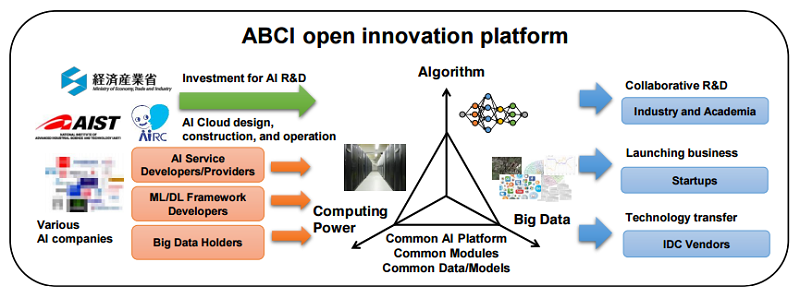
\includegraphics[width=5cm]{images/abci-innovation-800x298}
    \end{center}

    \begin{center}
      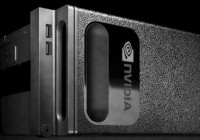
\includegraphics[width=3.5cm]{images/nvidia-dgx-1-bw-200x140}
    \end{center}
  \end{minipage}

  % \begin{itemize}
  % \item \textcolor{darkblue}{\textbf{Artificial Intelligence}} applications : e.g. \textbf{Japan} (ABCI: a 130 single precision PetaFlops system in late 2017) for Companies (book time for a fee)\\
  %   \textbf{AI Bridging Cloud Infrastructure}: goal is 43 (FP32) GigaFlops/Watt\\
  % \item \textcolor{darkgreen}{\textbf{Energy efficiency}}, e.g. \myhref{https://www.nextplatform.com/2016/11/14/nvidias-saturn-v-dgx-1-cluster-stacks/}{Nvidia's DGX-1 node} server (1 Dual Xeon + 8 GPU P100) aimed at deep learning ($\sim 18$ (FP64) GigaFlops/Watt).
  % \item Many new hardware solutions to come next year and after: Intel Knights Mill (XeonPhi, 3rd gen)
  % \end{itemize}

\end{frame}

%%%%%%%%%%%%%%%%%%%%%%%%%%%%%%%%%%%%%%%%%%%%%%%%%%%%%%%%%%%%%%%%%%%%%%%% 
%%%%%%%%%%%%%%%%%%%%%%%%%%%%%%%%%%%%%%%%%%%%%%%%%%%%%%%%%%%%%%%%%%%%%%%% 
\begin{frame}
  \frametitle{Supercomputer node architecture}

  \begin{center}
    \textbf{Multiples levels of hierarchy:}
    \begin{itemize}
    \item Need to aggregate the computing power of several 10 000 nodes !
    \item network efficiency: latency, bandwidth, topology
    \item memory: on-chip (cache), out-of-chip (DRAM), IO (disk)
    \item emmerging \textbf{hybrid programming model: MPI + X}
    \item \textcolor{red}{What is \textbf{X} ? OpenMP, OpenAcc, ..., \myhref{https://github.com/kokkos/kokkos}{Kokkos}, \myhref{https://github.com/llnl/raja}{RAJA}, ...}
    \item \textcolor{blue}{Even at node level MPI+X is required:} e.g. KNL
    \end{itemize}
  \end{center}

  \begin{figure}
    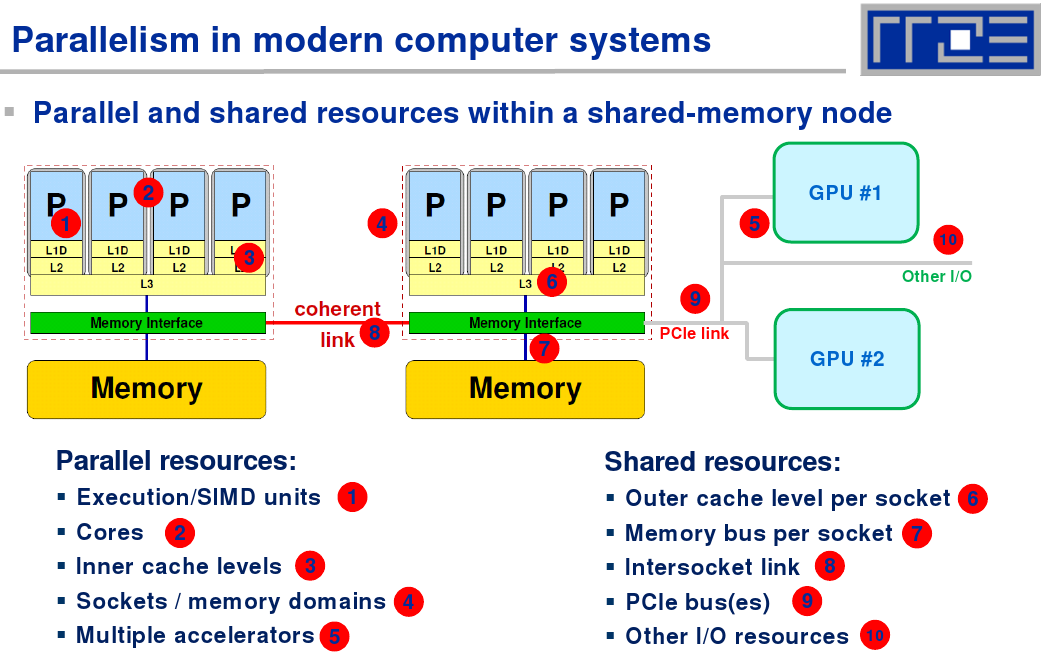
\includegraphics[width=5cm]{images/multicore_hardware}
    \caption{\scriptsize{Multi-core node summary,
        source: multicore tutorial (SC12) by G. Hager and G. Wellein}}
  \end{figure}
  
\end{frame}

%%%%%%%%%%%%%%%%%%%%%%%%%%%%%%%%%%%%%%%%%%%%%%%%%%%%%%%%%%%%%%%%%%%%%%%% 
%%%%%%%%%%%%%%%%%%%%%%%%%%%%%%%%%%%%%%%%%%%%%%%%%%%%%%%%%%%%%%%%%%%%%%%% 
% \begin{frame}
%   \frametitle{More heterogeneous  future...}

%   \begin{figure}
%     \includegraphics[height=6.5cm]{images/kokkos_heterogeneous}
%     \caption{
%       source: kokkos tutorial (GTC2014) by Carter Edwards}
%   \end{figure}
  
% \end{frame}


%%%%%%%%%%%%%%%%%%%%%%%%%%%%%%%%%%%%%%%%%%%%%%%%%%%%%%%%%%%%%%%%%%%%%%%% 
%%%%%%%%%%%%%%%%%%%%%%%%%%%%%%%%%%%%%%%%%%%%%%%%%%%%%%%%%%%%%%%%%%%%%%%% 
% \begin{frame}
%   \frametitle{What is a supercomputer ?}
  
%   % Power Efficiency over time
%   \begin{figure}
%     \includegraphics[height=6cm]{images/power_efficiency_horst_simon}
%     \caption{\myhref{http://www.extremetech.com/computing/155941-supercomputing-director-bets-2000-that-we-wont-have-exascale-computing-by-2020}{Horst Simon, LBNL}}
%   \end{figure}
  
% \end{frame}
